%% ============================================================================
%%  VLA Robot Learning — 5-Page Progress Report
%%  Compile: xelatex PROGRESS_REPORT.tex
%% ============================================================================
\documentclass[11pt, a4paper]{article}

\usepackage{fontspec}
\setmainfont{Helvetica Neue}
\setmonofont[Scale=0.85]{Menlo}
%% Fallback font for Unicode status symbols


\usepackage[left=0.80in, right=0.80in, top=0.75in, bottom=0.85in]{geometry}
\usepackage{setspace}
\setstretch{1.10}

\usepackage{graphicx}
\usepackage{amsmath, amssymb}
\usepackage{xcolor}
\usepackage{booktabs}
\usepackage{array}
\usepackage{tabularx}
\usepackage{enumitem}
\usepackage{multicol}
\usepackage{microtype}
\usepackage{parskip}
\setlength{\parskip}{2pt}
\usepackage{titlesec}
\usepackage{fancyhdr}
\usepackage{tcolorbox}
\tcbuselibrary{skins}

%% ── Colors ───────────────────────────────────────────────────────────────────
\definecolor{DarkGreen}  {HTML}{15803D}
\definecolor{FillGreen}  {HTML}{DCFCE7}
\definecolor{DimGray}    {HTML}{6B7280}
\definecolor{LightGray}  {HTML}{F3F4F6}
\definecolor{DarkGray}   {HTML}{374151}
\definecolor{AlertRed}   {HTML}{DC2626}
\definecolor{AlertAmber} {HTML}{D97706}
\definecolor{FillAmber}  {HTML}{FEF3C7}
\definecolor{EqnBg}      {HTML}{F0FDF4}
\definecolor{CodeBg}     {HTML}{F8FAFC}

%% ── Section style ────────────────────────────────────────────────────────────
\titleformat{\section}[block]
  {\large\bfseries\color{DarkGray}}{\thesection.}{0.5em}{}
  [\vspace{-5pt}{\color{DarkGreen}\rule{\linewidth}{1pt}}\vspace{1pt}]
\titlespacing{\section}{0pt}{8pt}{2pt}

\titleformat{\subsection}[block]
  {\normalsize\bfseries\color{DarkGray}}{\thesubsection}{0.5em}{}
\titlespacing{\subsection}{0pt}{5pt}{1pt}

%% ── Header / footer ──────────────────────────────────────────────────────────
\pagestyle{fancy}
\fancyhf{}
\fancyhead[L]{\small\textbf{\color{DarkGreen}VLA Robot Learning}
  \textcolor{DimGray}{--- Progress Report}}
\fancyhead[R]{\small\color{DimGray}Sara \& Connor · COMP 542}
\fancyfoot[C]{\small\color{DimGray}\thepage}
\renewcommand{\headrulewidth}{0.4pt}
\renewcommand{\footrulewidth}{0pt}

%% ── Coloured boxes ───────────────────────────────────────────────────────────
\newtcolorbox{pitchbox}{
  colback=FillGreen, colframe=DarkGreen, boxrule=1.2pt,
  arc=5pt, left=6pt, right=6pt, top=4pt, bottom=4pt,
}
\newtcolorbox{notebox}{
  colback=FillAmber, colframe=AlertAmber, boxrule=1pt,
  arc=4pt, left=6pt, right=6pt, top=3pt, bottom=3pt,
}
\newtcolorbox{eqnbox}{
  colback=EqnBg, colframe=DarkGreen!50, boxrule=0.8pt,
  arc=4pt, left=7pt, right=7pt, top=4pt, bottom=4pt,
}
\newtcolorbox{codebox}{
  colback=CodeBg, colframe=DimGray!40, boxrule=0.7pt,
  arc=3pt, left=5pt, right=5pt, top=3pt, bottom=3pt,
  fontupper=\footnotesize\ttfamily\color{DarkGray},
}

%% ── Column helpers ───────────────────────────────────────────────────────────
\newcolumntype{L}[1]{>{\raggedright\arraybackslash}p{#1}}
\newcolumntype{R}[1]{>{\raggedleft\arraybackslash}p{#1}}
\newcolumntype{C}[1]{>{\centering\arraybackslash}p{#1}}
\renewcommand{\arraystretch}{1.18}

%% ── Status symbols (using math/LaTeX, no Unicode) ────────────────────────────
\newcommand{\done}  {\textcolor{DarkGreen}{\textbf{$\checkmark$}}}
\newcommand{\pend}  {\textcolor{AlertRed}{$\circ$}}
\newcommand{\inprog}{\textcolor{AlertAmber}{$\bullet$}}

%% ============================================================================
\begin{document}
\thispagestyle{fancy}

%% ── Title block ──────────────────────────────────────────────────────────────
\begin{center}
  {\LARGE\bfseries\color{DarkGray} RLConditionedVLA}\\[3pt]
  {\large\color{DimGray}
    History-Conditioned Vision-Language-Action Model with RL Feedback}\\[6pt]
  \begin{tabular}{r@{\hspace{7pt}}l @{\hspace{22pt}} r@{\hspace{7pt}}l}
    \textbf{Authors}    & Sara Aly, Connor Juman &
    \textbf{Class}      & COMP 542 --- Machine Learning \\
    \textbf{Instructor} & Dr.\ Enno Huang        &
    \textbf{Date}       & March 2026 \\
  \end{tabular}
\end{center}
{\color{DimGray}\rule{\linewidth}{0.5pt}}

%% ============================================================================
\section{Main Idea \& Motivation}
%% ============================================================================

\begin{pitchbox}
\textbf{Core insight:} Standard VLA robot policies see only the current image
and a language goal --- they have no memory of what they already tried.
\textbf{RLConditionedVLA} encodes the history of past \emph{(action, reward)}
pairs as explicit input tokens, so the model can adapt its next action based
on whether recent attempts succeeded or failed, combining the perceptual
richness of vision-language models with the adaptive power of RL.
\end{pitchbox}

\vspace{3pt}

\begin{multicols}{2}
\setlength{\parskip}{1pt}

\subsection*{The Problem}
Existing VLA models such as RT-2 and Octo treat each timestep as an
independent mapping: \emph{image + instruction $\to$ action}.
Two critical signals are silently discarded at inference:
\begin{itemize}[leftmargin=1.1em, itemsep=0pt, topsep=1pt]
  \item \textbf{Failure history} --- the model cannot avoid repeating
        a failed action because it has no memory of prior attempts.
  \item \textbf{Reward signal} --- RL training optimises reward, yet the
        policy never observes reward at inference time.
  \item \textbf{Temporal self-model} --- without memory, the policy
        cannot plan across timesteps or recover from perturbations.
\end{itemize}

\columnbreak

\subsection*{Our Solution}
We fuse three input streams in a \textbf{causal Transformer}:
\begin{enumerate}[leftmargin=1.3em, itemsep=0pt, topsep=1pt]
  \item Video frames $\to$ CLIP ViT-B/32 $\to$ \texttt{vis\_proj}
  \item Language $\to$ CLIP Text Enc $\to$ \texttt{lang\_proj}
  \item $(a_i, r_i)_{i=t-H}^{t-1}$ $\to$ AR-History Encoder
\end{enumerate}
All projected to 256-dim tokens, assembled into a causal sequence, and
decoded into a discrete action via a 2-layer MLP head.
Training: (1)~behavioural cloning on expert demos, then (2)~online
REINFORCE fine-tuning under a KL penalty relative to the BC prior.
\end{multicols}

\vspace{2pt}
{\color{DimGray}\rule{\linewidth}{0.3pt}}
\vspace{2pt}

\begin{center}
\small\renewcommand{\arraystretch}{1.16}
\begin{tabular}{L{3.7cm} L{4.4cm} @{\hspace{8pt}} L{3.2cm} L{4.4cm}}
\toprule
\multicolumn{2}{c}{\textbf{Model Specification}} & \multicolumn{2}{c}{\textbf{Training Configuration}} \\
\midrule
Vision backbone   & CLIP ViT-B/32 (frozen, 86M)  & Phase 1       & Cross-entropy BC, $\epsilon{=}0.05$ label smoothing \\
Language backbone & CLIP Text Enc (frozen, 38M)  & Phase 2       & REINFORCE + value baseline + entropy + KL \\
History encoder   & AR-History Enc (trainable)   & Optimiser     & AdamW, lr $3{\times}10^{-4}$, cosine decay \\
Fusion module     & Causal Transformer 6L/8H     & Action space  & Discrete, $N$ actions (env-configurable) \\
Embed dim         & $d{=}256$, FFN dim $1024$    & History $H$   & 4 timesteps (ablated $\{0,1,2,4,8\}$) \\
Trainable params  & ${\approx}3.8\text{M}$ total & CLS token     & Last position (bug fix: was pos.~0) \\
\bottomrule
\end{tabular}
\end{center}

%% ============================================================================
\newpage
\section{System Architecture}
%% ============================================================================

\begin{figure}[h!]
\centering
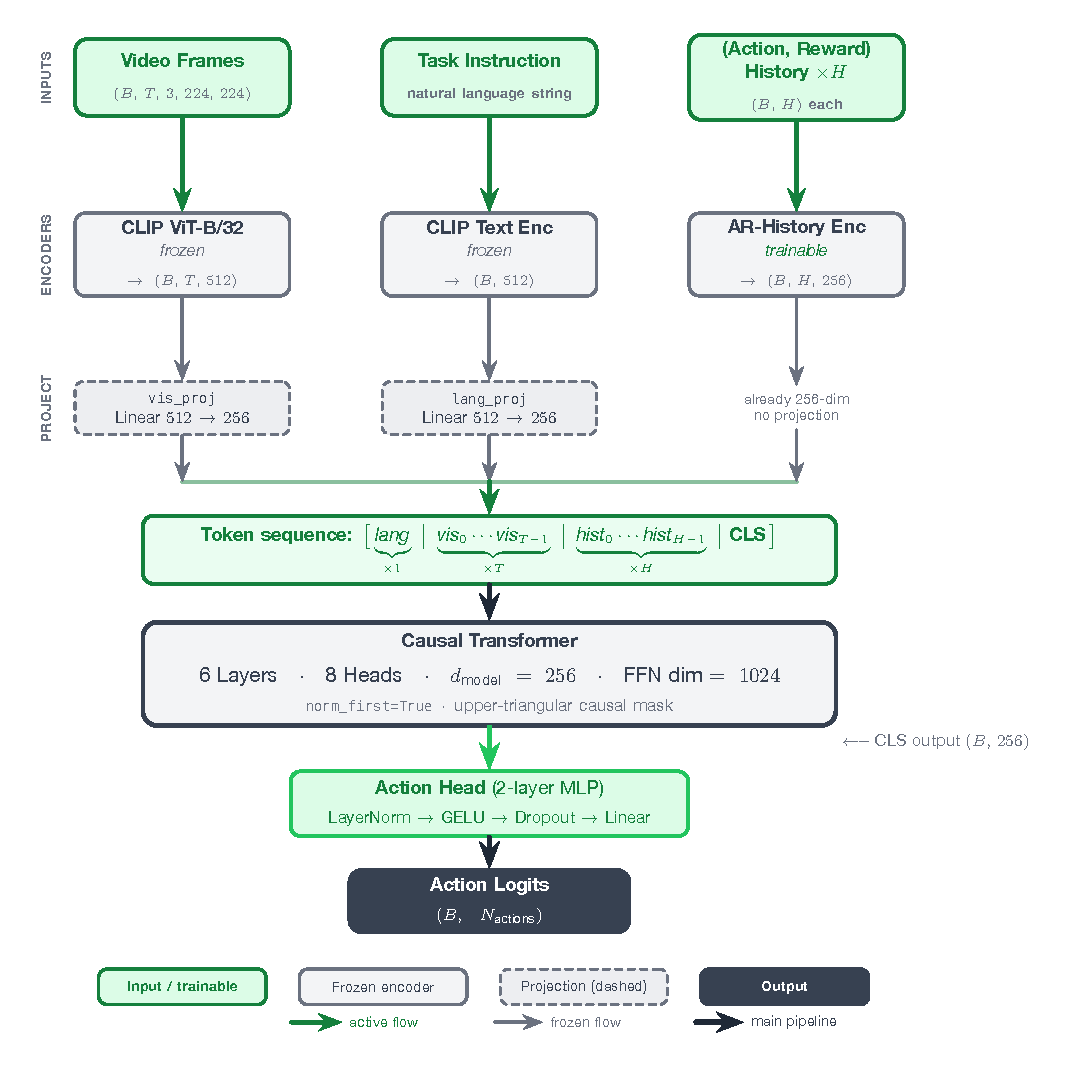
\includegraphics[width=\linewidth, height=0.43\textheight,
                 keepaspectratio]{architecture_diagram.pdf}
\caption{\small
  \textbf{RLConditionedVLA} forward pass.
  \textcolor{DarkGreen}{Green} = trainable; \textcolor{DimGray}{gray} = frozen CLIP.
  CLS is placed \emph{last} so the causal mask allows it to attend to every
  preceding token; its output is decoded by the action MLP head.}
\label{fig:arch}
\end{figure}

\vspace{3pt}

\begin{multicols}{2}
\setlength{\parskip}{2pt}

\subsection*{Design Rationale}

\textbf{Frozen CLIP encoders.}\enspace
CLIP ViT-B/32 and the CLIP text encoder provide strong representations
pre-trained on 400M image-text pairs.  Freezing them avoids catastrophic
forgetting and reduces trainable parameters to ${\approx}3.8$M, making
Phase 1 BC feasible on a single GPU.  Only the linear projection layers
(\texttt{vis\_proj}, \texttt{lang\_proj}: $512 \to 256$) are trained to
align CLIP features with the Transformer's token space.

\medskip
\textbf{Causal (not bidirectional) Transformer.}\enspace
The robot acts online: future rewards are unavailable when computing the
current action.  The upper-triangular causal mask enforces this inductive
bias and enables future extension to autoregressive multi-step action decoding.

\medskip
\textbf{Embedding table for actions.}\enspace
Naive integer encoding (action 3 = $3\times$ action 1) imposes a false
metric.  A learned table $\mathrm{Emb}(\cdot)\!\in\!\mathbb{R}^{(N{+}1)\times256}$
maps each action index to an independent dense vector.

\columnbreak

\textbf{CLS bug fix --- position 0 $\to$ last.}\enspace
The original implementation placed the CLS token at position 0.
Under a causal mask, position 0 attends only to itself --- no context.
Placing CLS at the \emph{last} position means it attends to every
language, visual, and history token.
This single fix significantly improved training convergence.

\medskip
\textbf{Two-phase training.}\enspace
Pure RL over discrete actions converges slowly with sparse rewards.
Phase 1 BC initialises the policy near the expert manifold; Phase 2 RL
fine-tunes it for higher return, with the KL penalty preventing
catastrophic drift from the BC prior.

\medskip
\textbf{Token sequence assembly.}\enspace
\[
  \mathbf{X}\!=\!\bigl[
    \underbrace{\mathbf{e}_\ell}_{1}
    \big|
    \underbrace{\mathbf{v}_{0:T-1}}_{T}
    \big|
    \underbrace{\mathbf{h}_{0:H-1}}_{H}
    \big|
    \underbrace{\mathbf{c}}_{\text{CLS}}
  \bigr]
  \!\in\!\mathbb{R}^{(1+T+H+1)\times256}
\]
$\mathbf{e}_\ell$ is placed first so all subsequent tokens attend to the
goal at every Transformer layer.  $\mathbf{h}_i$ encode recent
(action, reward) pairs (Eq.~2 on page~3).

\end{multicols}

%% ============================================================================
\newpage
\section{Key Equations \& Training Methodology}
%% ============================================================================

\subsection*{Mathematical Foundations}

\begin{eqnbox}
\small
\noindent
\begin{minipage}[t]{0.46\linewidth}

\textbf{(1)\;Policy formulation}
\begin{equation*}
  a_t = \arg\max_{a}\;\pi_\theta\!\left(
      a \;\middle|\; s_t,\;\ell,\;\mathcal{H}_t
  \right)
\end{equation*}
$\pi_\theta$: model parameterised by $\theta$;
$s_t$: current visual state;
$\ell$: language instruction;
$\mathcal{H}_t{=}\{(a_i,r_i)\}_{i=t-H}^{t-1}$: last $H$ step history.
$\arg\max$ selects the greedy action at inference.

\medskip
\textbf{(2)\;History token} for timestep $i$
\begin{equation*}
  \mathbf{h}_i = \mathrm{LN}\!\Bigl(
    \mathrm{Lin}\bigl[\mathrm{Emb}(a_i) \parallel W_r\,r_i\bigr]
    + \mathbf{p}_i
  \Bigr) \!\in\! \mathbb{R}^{256}
\end{equation*}
$\mathrm{Emb}(\cdot)\!\in\!\mathbb{R}^{(N+1)\times256}$: categorical lookup
so action identities are independent (no ordinal bias).
$W_r$: scalar reward projection.
$\mathbf{p}_i$: learnable positional embedding for slot~$i$.
$\mathrm{LN}$: LayerNorm for training stability.

\end{minipage}%
\hfill
\begin{minipage}[t]{0.49\linewidth}

\textbf{(3)\;Phase 1 --- Behavioural Cloning loss}
\begin{equation*}
  \mathcal{L}_{\mathrm{BC}} = -\sum_{c=1}^{N}
    \tilde{y}_c \,\log \hat{p}_c,
  \quad
  \tilde{y}_c = (1{-}\epsilon)\,y_c + \tfrac{\epsilon}{N}
\end{equation*}
$y_c\in\{0,1\}$: one-hot expert label;
$\hat{p}_c$: model softmax probability;
$\epsilon{=}0.05$: label smoothing preventing over-confident logits,
improving generalisation to unseen states.

\medskip
\textbf{(4)\;Phase 2 --- RL composite loss}
\begin{align*}
  \mathcal{L} =\;
    &\underbrace{-\mathbb{E}[\log\pi_\theta(a_t)\cdot\hat{A}_t]}_{\text{policy gradient}}
    +\underbrace{\tfrac{1}{2}(V(s_t)-G_t)^2}_{\text{value baseline}} \\[2pt]
    &-\underbrace{0.01\,\mathcal{H}[\pi_\theta]}_{\text{entropy bonus}}
    +\underbrace{0.1\,D_{\mathrm{KL}}(\pi_\theta \| \pi_{\mathrm{BC}})}_{\text{KL penalty}}
\end{align*}
$\hat{A}_t{=}G_t{-}V(s_t)$;
$G_t{=}\sum_{k\geq0}\gamma^k r_{t+k}$, $\gamma{=}0.99$;
$\pi_{\mathrm{BC}}$: frozen Phase~1 checkpoint.

\end{minipage}
\end{eqnbox}

\vspace{4pt}

\subsection*{Two-Phase Training Protocol}

\begin{center}
\small\renewcommand{\arraystretch}{1.16}
\begin{tabular}{L{2.4cm} L{4.6cm} L{4.6cm} L{3.1cm}}
\toprule
\textbf{Aspect} & \textbf{Phase 1 --- BC} & \textbf{Phase 2 --- RL} & \textbf{Rationale} \\
\midrule
Objective     & Supervised imitation of expert demos    & Maximise cumulative return $G_t$    & BC initialises policy \\
Loss          & Cross-entropy + label smoothing         & REINFORCE + value + entropy + KL    & RL refines from BC \\
Data          & Static demonstration dataset            & Online rollouts in environment      & Exploration needed \\
Frozen        & CLIP vision \& text encoders            & CLIP encoders + BC checkpoint       & Prevent forgetting \\
LR / stop     & $3{\times}10^{-4}$; val plateau         & $1{\times}10^{-4}$; KL $>$ 0.5 nats & Slower, stable RL \\
\bottomrule
\end{tabular}
\end{center}

\vspace{2pt}

\noindent\small\color{DimGray}
\textbf{Value head:}\enspace
$V(s_t)\!=\!\mathrm{MLP}_{\mathrm{val}}(\mathbf{c}_t)\!\in\!\mathbb{R}$ branches
off the same CLS output as the action head.  Advantage
$\hat{A}_t = G_t - V(s_t)$ reduces REINFORCE variance.
Entropy bonus encourages exploration; KL penalty acts as a trust-region
constraint preventing catastrophic drift from the BC prior.
\normalcolor\normalsize

%% ============================================================================
\newpage
\section{Implementation \& Codebase}
%% ============================================================================

\begin{multicols}{2}

\subsection*{Project Structure}

\begin{codebox}
RLConditionedVLA/\\
├── model/\\
│\ \ \ ├── vla\_model.py \ \ \ \ \ \ \# core model\\
│\ \ \ ├── history\_encoder.py \ \# AR-History Enc\\
│\ \ \ └── action\_head.py \ \ \ \ \# 2-layer MLP\\
├── training/\\
│\ \ \ ├── sft\_trainer.py \ \ \ \ \# Phase 1 BC\\
│\ \ \ ├── rl\_trainer.py \ \ \ \ \ \# Phase 2 RL\\
│\ \ \ └── trajectory\_dataset.py\\
├── envs/\\
│\ \ \ ├── gym\_wrapper.py \ \ \ \ \# Gymnasium API\\
│\ \ \ └── real\_robot\_stub.py \ \# hardware I/O\\
├── scripts/\\
│\ \ \ ├── train\_bc.py \ \ \# Phase 1 entry\\
│\ \ \ ├── train\_rl.py \ \ \# Phase 2 entry\\
│\ \ \ └── evaluate.py \ \ \# policy eval\\
├── config.yaml \ \ \ \ \ \ \ \# hyperparams\\
└── generate\_report.py \ \# PDF builder
\end{codebox}

\columnbreak

\subsection*{Key Implementation Details}

\textbf{CLIP integration.}\enspace
Both CLIP encoders are loaded via HuggingFace \texttt{transformers} and
frozen immediately after loading.  Only the two linear projection layers
(\texttt{vis\_proj}, \texttt{lang\_proj}: $512 \to 256$) are trainable.

\medskip
\textbf{Causal Transformer.}\enspace
A 6-layer, 8-head self-attention stack with Pre-LayerNorm for training
stability.  The upper-triangular causal mask is generated once per batch,
ensuring each token only attends to prior positions.

\medskip
\textbf{History padding.}\enspace
At episode start, history slots are filled with a \texttt{<PAD>} action
token (index $N$) and reward $= 0.0$, giving the model a neutral but
valid history from timestep~0.

\medskip
\textbf{Gymnasium wrapper.}\enspace
\texttt{gym\_wrapper.py} converts any Gymnasium-compatible environment
into the step signature expected by the RL trainer.  Images are resized to
$224{\times}224$ and normalised with CLIP's mean/std before \texttt{vis\_proj}.

\medskip
\textbf{Report compilation.}\enspace
\texttt{generate\_report.py --tex} automates two xelatex passes plus bibtex
for cross-references.

\end{multicols}

\vspace{3pt}

\subsection*{Configurable Hyperparameters (\texttt{config.yaml})}

\begin{center}
\footnotesize\renewcommand{\arraystretch}{1.16}
%% Column widths: 2.8+1.5+3.5 + gap + 2.8+1.5+1.8 = 14.4cm + ~1.9cm separators = 16.3cm (fits 16.9cm)
\begin{tabular}{L{2.8cm} C{1.5cm} L{3.5cm} @{\hspace{6pt}} L{2.8cm} C{1.5cm} L{1.8cm}}
\toprule
\textbf{Parameter} & \textbf{Default} & \textbf{Description} &
\textbf{Parameter} & \textbf{Default} & \textbf{Role} \\
\midrule
\texttt{history\_len}    & 4      & History window $H$      & \texttt{d\_model}      & 256   & Token dim  \\
\texttt{n\_actions}      & env    & Discrete action count   & \texttt{n\_heads}      & 8     & Attn heads \\
\texttt{lr\_phase1}      & 3e-4   & BC learning rate        & \texttt{n\_layers}     & 6     & Depth      \\
\texttt{lr\_phase2}      & 1e-4   & RL learning rate        & \texttt{ffn\_dim}      & 1024  & FFN width  \\
\texttt{label\_smooth}   & 0.05   & BC smoothing $\epsilon$ & \texttt{dropout}       & 0.1   & Reg.       \\
\texttt{kl\_coeff}       & 0.1    & KL penalty weight       & \texttt{gamma}         & 0.99  & Discount   \\
\texttt{entropy\_coeff}  & 0.01   & Entropy bonus weight    & \texttt{clip\_grad}    & 1.0   & Grad clip  \\
\bottomrule
\end{tabular}
\end{center}

%% ============================================================================
\newpage
\section{Current Progress \& Roadmap}
%% ============================================================================

\begin{notebox}
\small
\textbf{Status --- March 2026.}\enspace
All core model and training infrastructure is complete and verified on
synthetic end-to-end data.  The codebase runs on CPU and CUDA (tested on
RTX 3090).  Remaining work: environment selection, demonstration collection,
and both training phases with full logging and ablation studies.
\end{notebox}

\vspace{4pt}

\begin{center}
\footnotesize\renewcommand{\arraystretch}{1.14}
\begin{tabular}{L{5.3cm} c @{\hspace{10pt}} L{5.3cm} c}
\toprule
\textbf{Component} & \textbf{Status} & \textbf{Component} & \textbf{Status} \\
\midrule
\texttt{RLConditionedVLA} model class    & \done   & Evaluation script (\texttt{evaluate.py}) & \done   \\
\texttt{ActionRewardHistoryEncoder}      & \done   & Config file (\texttt{config.yaml})        & \done   \\
CLS bug fix (pos.~0 $\to$ last)          & \done   & Gymnasium sim wrapper                    & \done   \\
BC trainer (\texttt{sft\_trainer.py})   & \done   & Real robot interface stub                 & \done   \\
RL trainer (\texttt{rl\_trainer.py})    & \done   & Architecture diagram (TikZ/PDF)          & \done   \\
Value head + advantage estimation        & \done   & Full PDF reports (this document)         & \done   \\
Trajectory dataset loader                & \done   & \texttt{generate\_report.py --tex} flag  & \done   \\
Label smoothing + KL penalty             & \done   & TensorBoard logging integration           & \inprog \\
Synthetic end-to-end smoke test          & \done   & Environment selection                     & \inprog \\
                                         &         & Demonstration data collection             & \pend   \\
                                         &         & Phase 1 (BC) training run                 & \pend   \\
                                         &         & Phase 2 (RL) training run                 & \pend   \\
                                         &         & Ablation studies ($\times$6 conditions)   & \pend   \\
                                         &         & Sim-to-real transfer evaluation           & \pend   \\
\bottomrule
\multicolumn{4}{r}{\textcolor{DarkGreen}{\done}\ Done\quad
                   \textcolor{AlertAmber}{\inprog}\ In progress\quad
                   \textcolor{AlertRed}{\pend}\ Pending}\\
\end{tabular}
\end{center}

\vspace{4pt}

\subsection*{Planned Ablation Studies}

\begin{center}
\footnotesize\renewcommand{\arraystretch}{1.16}
\begin{tabular}{C{0.5cm} L{4.0cm} L{5.2cm} L{4.9cm}}
\toprule
\textbf{\#} & \textbf{Condition} & \textbf{Modification} & \textbf{Tests} \\
\midrule
A1 & No history ($H{=}0$)   & Remove history encoder; lang + vision only        & Value of history conditioning \\
A2 & No reward in history    & Pass only action index; $r_i{=}0$ always          & Value of reward signal \\
A3 & History length sweep    & $H \in \{1, 2, 4, 8\}$ (four runs)               & Optimal context window size \\
A4 & BC only (no RL)         & Skip Phase 2; evaluate Phase 1 checkpoint         & Benefit of RL fine-tuning \\
A5 & No KL penalty           & Set $\lambda_{\mathrm{KL}}{=}0$ in Phase 2        & Stability of trust-region \\
A6 & PPO vs.\ REINFORCE      & Replace REINFORCE with PPO clipped objective      & Sample efficiency \\
\bottomrule
\end{tabular}
\end{center}

\vspace{4pt}

\subsection*{Immediate Next Steps}

\begin{enumerate}[leftmargin=1.5em, itemsep=0pt, topsep=1pt]
  \item \textbf{Select environment.}
        Evaluate \texttt{MiniGrid-Empty-5x5} vs.\ \texttt{FetchReach-v2};
        update \texttt{config.yaml} with $N$, image resolution, reward shaping.

  \item \textbf{Collect demonstrations.}
        Scripted policy; ${\geq}500$ episodes $\to$ \texttt{data/episodes.pkl}.

  \item \textbf{Phase 1 (BC).}
        Target val accuracy $\geq 3\times$ random ($= 1/N$);
        TensorBoard logging; checkpoint every 5 epochs.

  \item \textbf{Phase 2 (RL).}
        Init from best Phase 1; stop if $D_{\mathrm{KL}} > 0.5$ nats
        for 3 consecutive epochs.

  \item \textbf{Ablations A1--A6} (one modification each; 5 seeds per condition).

  \item \textbf{Final report:} results tables, learning curves, ablation charts.
\end{enumerate}


\end{document}
